\documentclass[twocolumn,10pt]{article}
\usepackage[a4paper, top=1.0in, bottom=1.0in, left=0.85in, right=0.85in]{geometry}

\usepackage{graphicx}
\usepackage{algorithm}  
\usepackage{algorithmicx}  
\usepackage{algpseudocode}  
\usepackage{amsmath}
\usepackage{url}

\renewcommand{\algorithmicrequire}{\textbf{Input:}}  
\renewcommand{\algorithmicensure}{\textbf{Output:}}  
\graphicspath{{figure/}}

\begin{document}

\date{November 17th, 2016}

\title{\bf A Web Crawler Design for Plant Data Collection}

\author{
	201620700 Xiang, Qin
	\\ Advisor Li, Jie
}

\maketitle

\section{Introduction}
A web crawler\cite{olston2010web} (also known as a robot or a spider) is a system for the bulk downloading of web pages. Web crawlers are used for a variety of purposes. Most prominently, they are one of the main components of web search engines, systems that assemble a corpus of web pages, index them, and allow users to issue queries against the index and find the web pages that match the queries. A related use is web archiving, where large  sets of web pages are periodically collected and archived for posterity. A third use is web data mining, where web pages are analyzed for statistical properties, or where data analytics is performed on them. Finally, web monitoring services allow their clients to submit standing queries, or triggers, and they continuously crawl the web and notify clients of pages that match those queries.\par
The basic flow of web crawler is shown in Figure 1. This is a sequential example. The starting pages are called seed. Web crawler starts to crawl from seed. Then in the crawl process, we may have a list, sometimes called frontier, to crawl. Every time we extract one URL from the list, access the URL to get the information in it. After that, we may add URLs into the frontier. To analyze the data, we need to store the information we crawled from the pages into the repository, like database.  At last we may need a check to determine when to stop crawling.\par
\begin{figure}
	\centering
	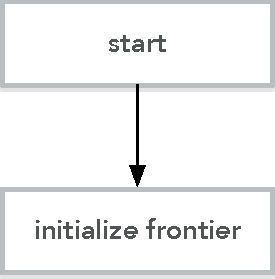
\includegraphics[width = 0.2\textwidth]{figure1}
	\caption{Basic Flow of Web Crawler}
\end{figure}
There are two normal search strategies.  One is Breadth-first search(Figure 2), the other is Depth-first search(Figure 3). Breadth-first search can be implemented by queue, which uses the FIFO(First In, First Out). And Depth-first search can be implemented by the stack(LIFO) or recursion.\par
\begin{figure}
	\centering
	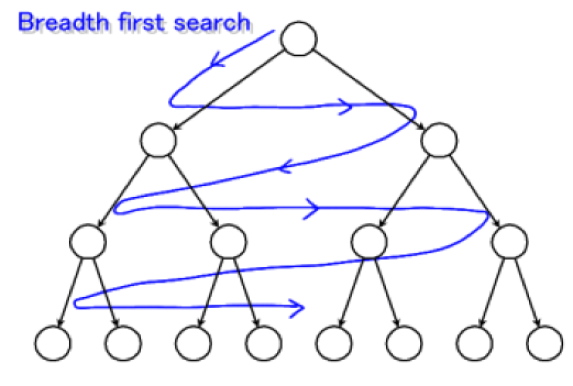
\includegraphics[width = .3\textwidth]{pic2.png}
	\caption{Breadth-first Search}
\end{figure}
\begin{figure}
	\centering
	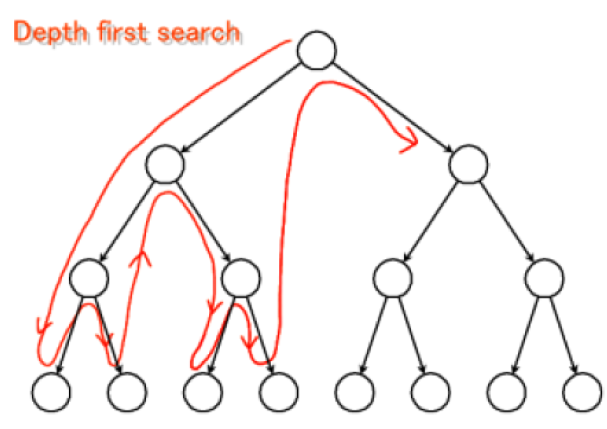
\includegraphics[width = .3\textwidth]{pic3.png}
	\caption{Depth-first Search}
\end{figure}
Another existed method is originally used to looking for external links of one page. I intend to use it not only for searching for external links, but also searching for the data about plant. And then store the data in database, clean the data. At last, I intend to make an analysis about the collected data. So, I make changes of the existed method, let it grab the data from pages, not just links. When crawling job of one page is finished, it will ask if we need to continue crawling. What's more, I add some checks on the links, so that the program will not crash.\par
\section{Related Research}
\subsection{BeautifulSoup}
The BeautifulSoup is a function library, which tries to make sense of the nonsensical; it helps format and organize the messy web by fixing bad HTML and presenting us with easily-traversible Python objects representing XML structures. For instance, the BeautifulSoup can transform a html page into a BeautifulSoup object, with the following structure(Figure 4):\par
\begin{figure}
	\centering
	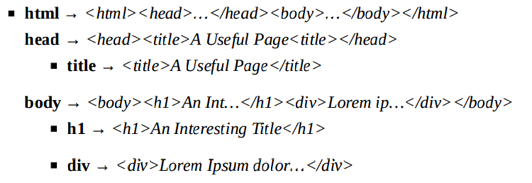
\includegraphics[width = .3\textwidth]{pic4.png}
	\caption{Parsed by BeautifulSoup}
\end{figure}
\subsection{Regular expressions in Python}
A regular expression, regex or regexp is a sequence of characters that define a search pattern. Usually this pattern is then used by string searching algorithms for "find" or "find and replace" operations on strings. The Figure 5 lists some commonly used regular expression symbols, with a brief explanation and example. These 12 symbols are the most commonly used regular expressions in Python, and can be used to find and collect most any string type. A regular expression can be inserted as any argument in a BeautifulSoup expression, allowing you a flexibility in finding target elements.\par
\begin{figure}
	\centering
	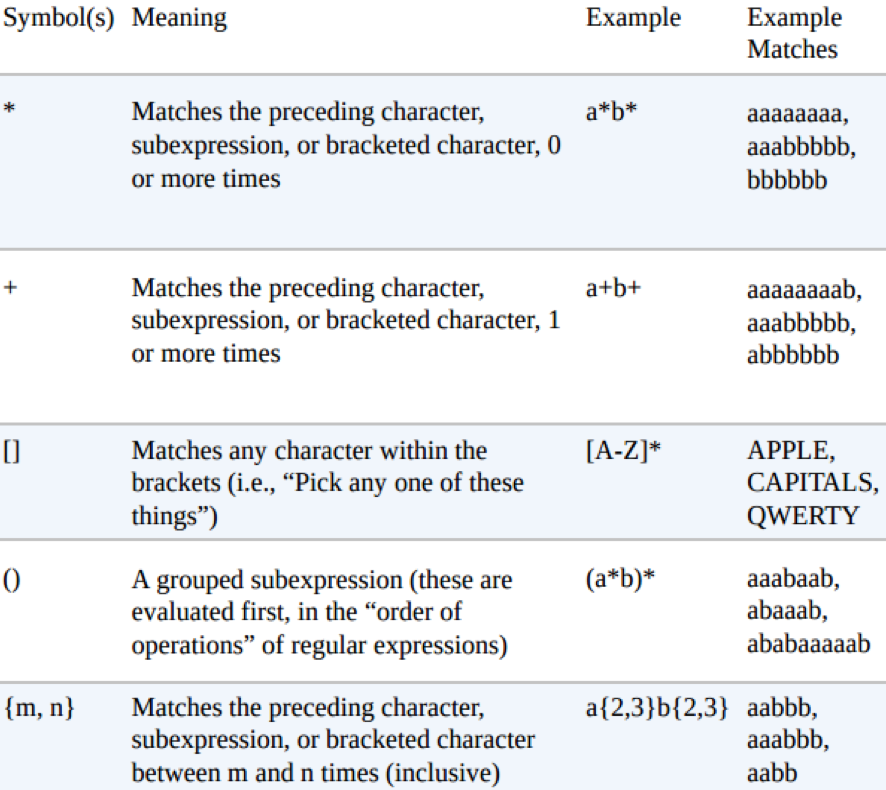
\includegraphics[width = .3\textwidth]{pic5.png}
	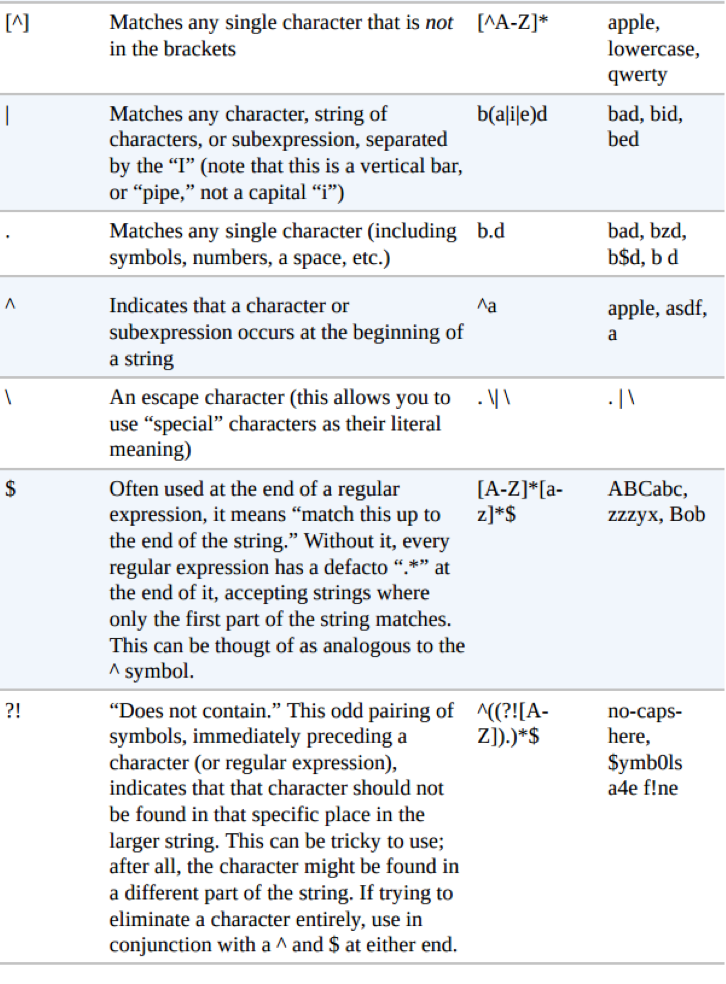
\includegraphics[width = .3\textwidth]{pic5-2.png}
	\caption{Common Regular Expressions}
\end{figure}
\section{System Description}
\subsection{Purpose}
There are two purposes to run this experiment:\par
- Make a web crawler to crawl the information about the plant. And then store the data in the local database.\par
- Analyze the local data and make a prediction from the data, like climate.
\subsection{Proposed Model}
Suppose that we intend to crawl the Internet from one starting page. We hope to grab all the information about this page, including its internal links and external links. After all the contents from this page, if we need to crawl more pages, we can start from one of its external links and continue this process. The basic flow is shown in Figure 6:\par
\begin{figure}
	\centering
	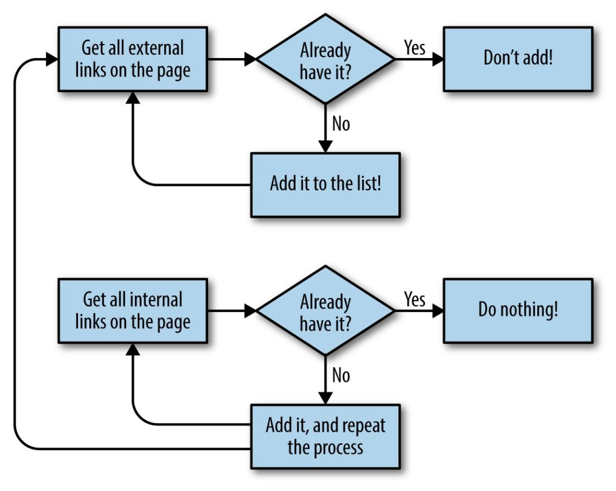
\includegraphics[width = .3\textwidth]{pic6.png}
	\caption{The Stratege of Crawl}
\end{figure}
There are two loops in this method. One is to get the internal links. The other is to get the external links. I let it get the contents of the pages while it access a new page. And make a list to record the footprints. So that it will not access the same page again. And if we intend to continue crawling after all the internal links and external links are found, then a new starting page will begin from one of its external links. Furthermore, I add error checks on links and set the crawling interval to 1 second.
\subsection{Results}
\begin{figure}
	\centering
	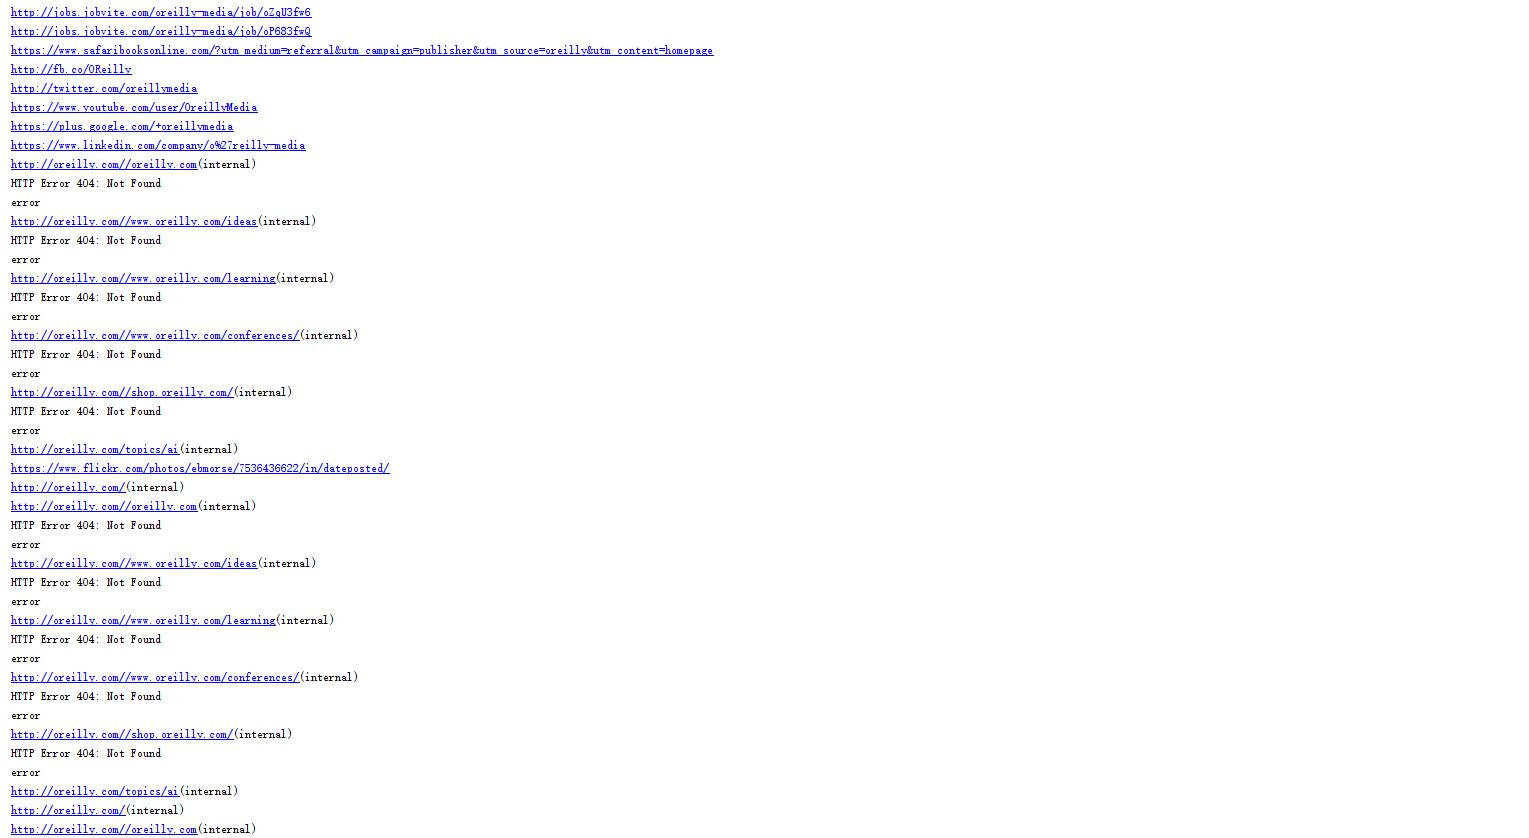
\includegraphics[width = .4\textwidth]{r3.png}
	\caption{Crawling}
\end{figure}
\begin{figure}
	\centering
	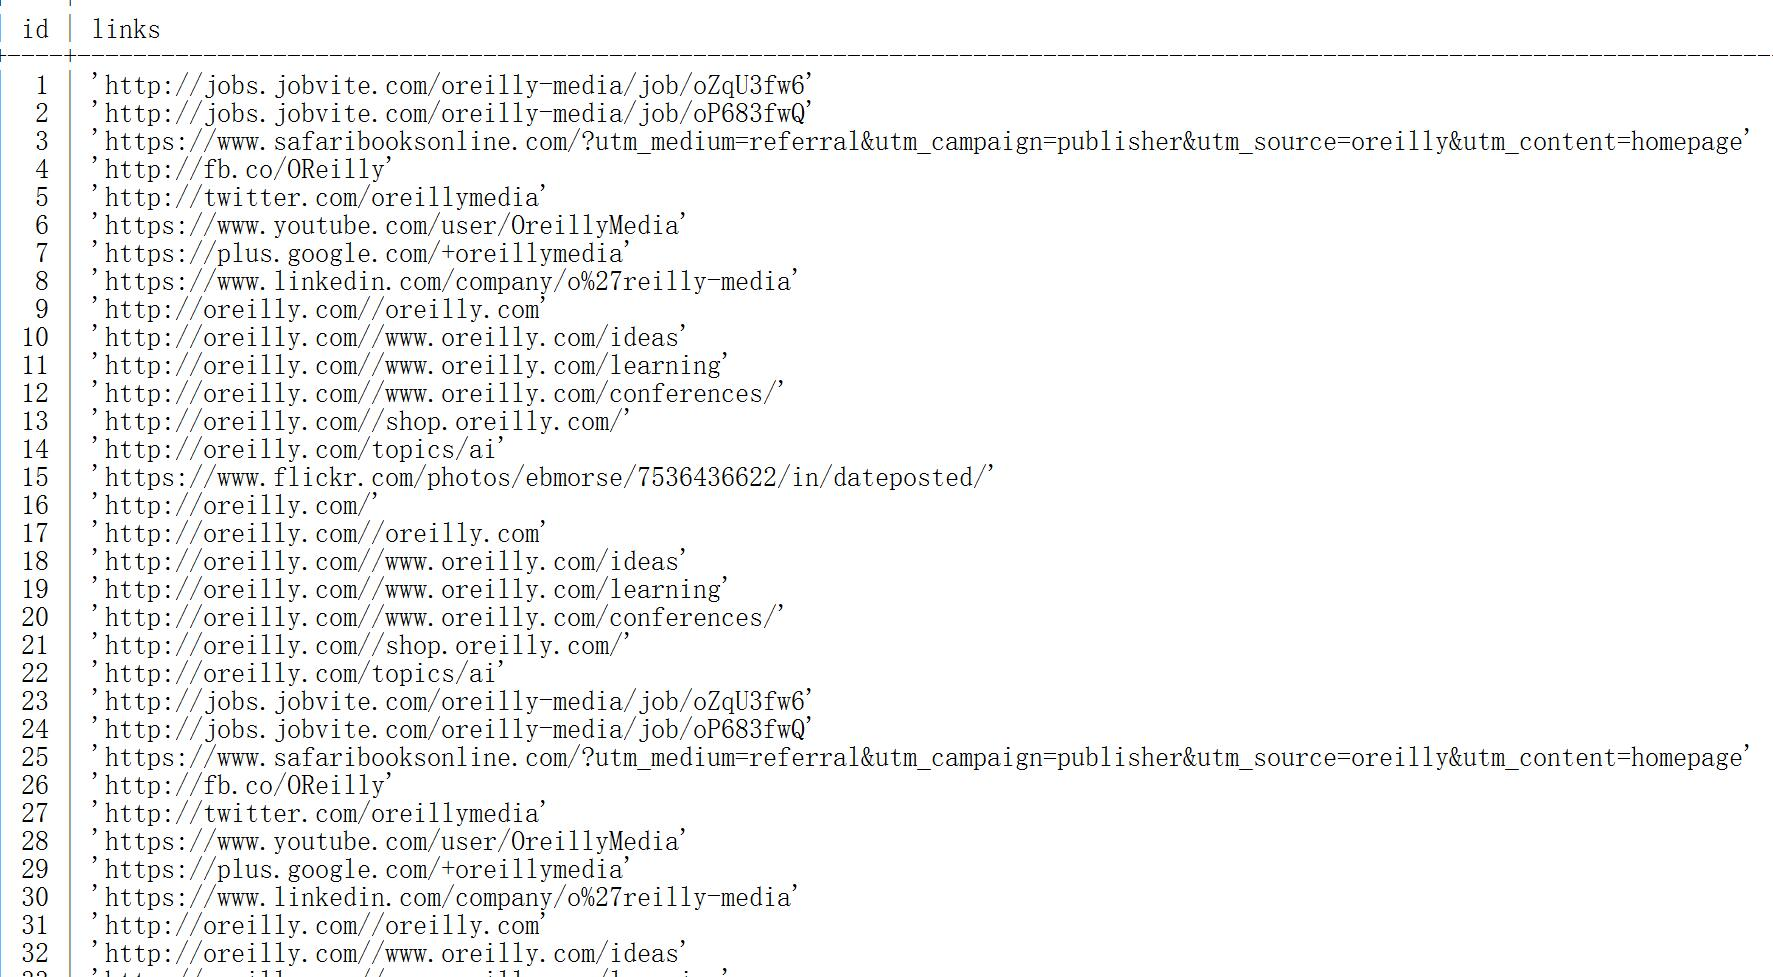
\includegraphics[width = .4\textwidth]{r2.png}
	\caption{Storing in database}
\end{figure}
Results are shown in Figure 7 and Figure 8. To show the results, here only the links are collected, as there are still some challenges to be done. Like parse the contents in the pages. Also it is preferred to store more effictive data in database, not just copy all the contents of them.
\section{Evaluation}
There are some merits about this method:\par
- It can reduce redundancy with a list to record the already accessed pages.\par
- To avoid unexpected error, there are checks to make sure it will not crush. Such as HTTP errors, server is not found and attributes of tag is not existed.\par
- To reduce the overhead to the network, the crawl is run at regular intervals.\par
\section{Future Work}
Eventhough we can get the links and print the pages,
there are still some challenges are needed to be solved:\par
- How to parse the web pages we get. For example, deal with the increasing file format, like: PDF, Flash, SVG, RSS.\par
- Given finite storage capacity, in practice crawlers discard or retire low-quality and spam pages from their collections, to make room for superior pages.\par
- How to deal with dynamic pages.\par
- How to avoid violating the law.\par
- The way of storage in database.\par
- Python set a recursion limit to 1000 times. What to do if it reach the maximun recursion depth.\par
- How to grab picture an video.\par
- How to deal with the repeating segments appeared in URLs, like:$/blog/blog/blog/blog.../blog/title_of_blog.php$\par
- Clean the data once in the database.\par
What's more, the crawling method may be improved in several ways. After finishing the tasks, how to analyze the data is still a problem to be done.

\begin{table}[tbp]
	\centering  
	\begin{tabular}{lll}  
		\hline
		Column &Data Type & Introduction\\ 
		\hline  
		sid &String & Physical unique identifier\\
		content & String & JSON String of object\\ 
		object & String & Name of object\\
		count & Integer16 & Count of sync time\\
		resend & Boolean &Necessity of resending data \\
		sendtime & Date & Data send time\\
		\hline
	\end{tabular}
	\caption{Columns of sender table}
\end{table}

\bibliographystyle{unsrt}
{
	\footnotesize
	\bibliography{ref}
}

\end{document}
